% Generated by ArticleSignalDiagrams. Opaque vector fills only.
\documentclass[10pt,tikz,border=5pt]{standalone}
\usepackage{lmodern}
\usetikzlibrary{fit}
\begin{document}
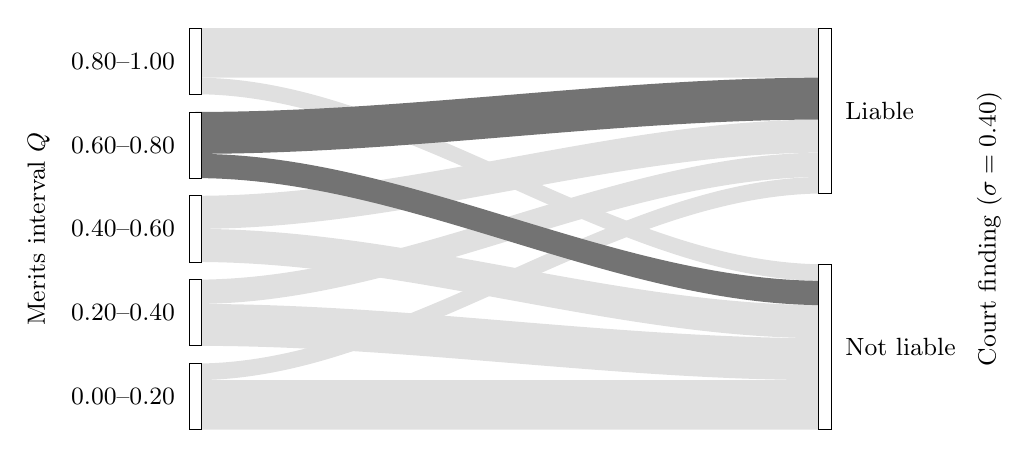
\begin{tikzpicture}[x=1cm,y=1cm,font=\small]\path[fill=black!12,draw=none] (3.3,-5.1) .. controls (6,-5.1) and (8.6,-5.1) .. (11.3,-5.1) -- (11.3,-4.470699) .. controls (8.6,-4.470699) and (6,-4.470699) .. (3.3,-4.470699) -- cycle;
\path[fill=black!12,draw=none] (3.3,-4.470699) .. controls (6,-4.470699) and (8.6,-2.1) .. (11.3,-2.1) -- (11.3,-1.889301) .. controls (8.6,-1.889301) and (6,-4.26) .. (3.3,-4.26) -- cycle;
\path[fill=black!12,draw=none] (3.3,-4.035) .. controls (6,-4.035) and (8.6,-4.470699) .. (11.3,-4.470699) -- (11.3,-3.938869) .. controls (8.6,-3.938869) and (6,-3.503171) .. (3.3,-3.503171) -- cycle;
\path[fill=black!12,draw=none] (3.3,-3.503171) .. controls (6,-3.503171) and (8.6,-1.889301) .. (11.3,-1.889301) -- (11.3,-1.581131) .. controls (8.6,-1.581131) and (6,-3.195) .. (3.3,-3.195) -- cycle;
\path[fill=black!12,draw=none] (3.3,-2.97) .. controls (6,-2.97) and (8.6,-3.938869) .. (11.3,-3.938869) -- (11.3,-3.518869) .. controls (8.6,-3.518869) and (6,-2.55) .. (3.3,-2.55) -- cycle;
\path[fill=black!12,draw=none] (3.3,-2.55) .. controls (6,-2.55) and (8.6,-1.581131) .. (11.3,-1.581131) -- (11.3,-1.161131) .. controls (8.6,-1.161131) and (6,-2.13) .. (3.3,-2.13) -- cycle;
\path[fill=black!12,draw=none] (3.3,-0.84) .. controls (6,-0.84) and (8.6,-3.210699) .. (11.3,-3.210699) -- (11.3,-3) .. controls (8.6,-3) and (6,-0.629301) .. (3.3,-0.629301) -- cycle;
\path[fill=black!12,draw=none] (3.3,-0.629301) .. controls (6,-0.629301) and (8.6,-0.629301) .. (11.3,-0.629301) -- (11.3,-0) .. controls (8.6,-0) and (6,-0) .. (3.3,-0) -- cycle;
\path[fill=black!55,draw=none] (3.3,-1.905) .. controls (6,-1.905) and (8.6,-3.518869) .. (11.3,-3.518869) -- (11.3,-3.210699) .. controls (8.6,-3.210699) and (6,-1.596829) .. (3.3,-1.596829) -- cycle;
\path[fill=black!55,draw=none] (3.3,-1.596829) .. controls (6,-1.596829) and (8.6,-1.161131) .. (11.3,-1.161131) -- (11.3,-0.629301) .. controls (8.6,-0.629301) and (6,-1.065) .. (3.3,-1.065) -- cycle;
\coordinate (axis-midline-0) at (0,-2.55);
\path[fill=white,draw=black,line width=0.3pt] (3.22,-5.1) rectangle (3.38,-4.26);
\node[anchor=east,fill=white,inner sep=2pt] (bucket-0-0-0) at (3.12,-4.68) {0.00--0.20};
\path[fill=white,draw=black,line width=0.3pt] (3.22,-4.035) rectangle (3.38,-3.195);
\node[anchor=east,fill=white,inner sep=2pt] (bucket-0-0-1) at (3.12,-3.615) {0.20--0.40};
\path[fill=white,draw=black,line width=0.3pt] (3.22,-2.97) rectangle (3.38,-2.13);
\node[anchor=east,fill=white,inner sep=2pt] (bucket-0-0-2) at (3.12,-2.55) {0.40--0.60};
\path[fill=white,draw=black,line width=0.3pt] (3.22,-1.905) rectangle (3.38,-1.065);
\node[anchor=east,fill=white,inner sep=2pt] (bucket-0-0-3) at (3.12,-1.485) {0.60--0.80};
\path[fill=white,draw=black,line width=0.3pt] (3.22,-0.84) rectangle (3.38,-0);
\node[anchor=east,fill=white,inner sep=2pt] (bucket-0-0-4) at (3.12,-0.42) {0.80--1.00};
\node[fit=(bucket-0-0-0) (bucket-0-0-1) (bucket-0-0-2) (bucket-0-0-3) (bucket-0-0-4),inner sep=0pt] (source-labels-0) {};
\coordinate (axis-title-0-0) at (source-labels-0.west |- axis-midline-0);
\node[rotate=90,anchor=south,inner sep=0pt] at ([xshift=-0.18cm]axis-title-0-0) {Merits interval $Q$};
\path[fill=white,draw=black,line width=0.3pt] (11.22,-5.1) rectangle (11.38,-3);
\node[anchor=west,fill=white,inner sep=2pt] (bucket-0-1-0) at (11.48,-4.05) {Not liable};
\path[fill=white,draw=black,line width=0.3pt] (11.22,-2.1) rectangle (11.38,0);
\node[anchor=west,fill=white,inner sep=2pt] (bucket-0-1-1) at (11.48,-1.05) {Liable};
\node[fit=(bucket-0-1-0) (bucket-0-1-1),inner sep=0pt] (destination-labels-0) {};
\coordinate (axis-title-0-1) at (destination-labels-0.east |- axis-midline-0);
\node[rotate=90,anchor=north,inner sep=0pt] at ([xshift=0.18cm]axis-title-0-1) {Court finding ($\sigma=0.40$)};
\end{tikzpicture}
\end{document}

